\documentclass{article}
\usepackage[utf8]{inputenc}

\title{Adversarial Label Smoothing}
\author{Morgane Goibert$\quad\quad\quad\quad$Elvis Dohmatob}
\date{February 2019}

\usepackage{amsmath,amsfonts,amssymb,amsthm}
\usepackage{hyperref}
\usepackage{natbib}
\usepackage{authblk}
\usepackage{graphicx,color}
\usepackage{subfig}
\usepackage{mdframed}
\usepackage{bbold}
\usepackage{comment}


\newtheorem{theorem}{Theorem}
\newtheorem{lemma}{Lemma}
\newtheorem{assumption}{Assumption}
\newtheorem{corollary}{Corollary}
\newtheorem{conjecture}{Conjecture}
\newtheorem{proposition}{Proposition}
\newtheorem{hypothesis}{Hypothesis}
\theoremstyle{definition}
\newtheorem{remark}{Remark}
\newtheorem{definition}{Definition}

\DeclareMathOperator{\hell}{Hell}
\DeclareMathOperator{\tv}{TV}
\DeclareMathOperator{\wass}{W_1}
\DeclareMathOperator{\argmax}{argmax}
\DeclareMathOperator{\argmin}{argmin}
\DeclareMathOperator{\bern}{Bernoulli}
\DeclareMathOperator{\unif}{U}
\DeclareMathOperator{\tri}{Tri}
\DeclareMathOperator{\acc}{Acc}
\DeclareMathOperator{\li}{Li}
\providecommand{\todo}[1]{\textbf{\textcolor{red}{#1}}}

\begin{document}

\maketitle

\begin{abstract}
  Woof!
\end{abstract}
\tableofcontents
\section{Introduction}
At a very high-level, the only information provided by the label $y$ of an input
$x$ is that of all the other possible labels $y' \in [\![k]\!]$, $y$ is the most
befitting.

\subsection{Notations}
Labels are
denoted $y, y_i \in [\![k]\!]$, and the corresponding one-hot encodings are
denoted $\delta_{y},\delta_{y_i} \in \Delta_k$. For a class $j \in [\![K]\!]$,
$q(j)$ is the $j$ component of a vector $q \in \mathbb R^k$. For a neural net
$\theta$, $z(j|x;\theta)$ denotes the the $j$ component of the logit for input
$x$. $p(j|x)=\exp(z|x;\theta)/\sum_{k}\exp(z|x;\theta)$ is the softmax
distribution on the classes $j\in[\![K]\!]$.

\section{Contributions}
\subsection{Adversarial label smoothing}
Let $\tv(\cdot\|\cdot)$ be the Total-Variation distance  defined by $\tv(q\|p)
:= (1/2)\|q-p\|_1$. Let $\hat{P}_n := \frac{1}{n}\sum_{i=1}\delta_{x_i} \otimes
\delta_{y_i}$ be the empirical distribution of the input-label pairs $(x,y)$ in
the dataset. For an uncertainty tolerance level $\epsilon>0$, define the
uncertainty set
\begin{eqnarray}
  \begin{split}
    \mathcal U_\epsilon(\hat{P}_n) &:= \{P_XQ_{Y|X} |
  \tv(Q_{Y|x}\|\hat{P}_n(\cdot|x)) \le \epsilon,\;\forall x \in \mathcal X\}\\
  &=\left\{\sum_{i=1}^n(1/n)\delta_{x_i} \otimes q_i | q_i \in \Delta_k,\;
    \tv(q_i\|\delta_{y_i})\le \epsilon\;\forall i \in [\![n]\!]\right\},
  \end{split}
\end{eqnarray}
made up of joint distributions $Q \in \mathcal P(\mathcal X \times \mathcal Y)$
on input-label pairs $(x_i,y_i)$, for which the marginal label distribution
$q_i:=Q_{Y|X=x_i} \in \mathcal P(\mathcal Y)=\Delta_k$ is within  TV distance
$\le \epsilon$ of the one-hot encoding of the observed label $\delta_{y_i}$. By
direct computation, one has
$$
\tv(q_i\|\delta_{y_i}) = (1/2)\sum_{j=1}^k|q_i(j)-\delta_{y_i}(j)| = (1/2)
\left(\sum_{j \ne y_i}q_i(j) + 1 - q_i(y_i)\right)=1-q_i(y_i),
$$
and so the uncertainty set can be rewritten as
\begin{eqnarray}
  \mathcal U_\epsilon(\hat{P}_n)=\left\{\sum_{i=1}^n(1/n)\delta_{x_i} \otimes q_i | q_i \in
  \Delta_k,\;q_i(y_i)\ge 1 - \epsilon\;\forall i \in [\![n]\!]\right\}.
\end{eqnarray}



Now, consider the two-player game
\begin{eqnarray}
  \begin{split}
    \min_{\theta}\max_{Q \in \mathcal U_\epsilon(\hat{P}_n)} \mathbb E_{(x,y)
      \sim Q}[-\delta_y^T\log(p(\cdot|x;\theta))].
  \end{split}
  \label{eq:grand}
\end{eqnarray}
Mindful of the previous computations, one has
\begin{eqnarray}
  \begin{split}
    \min_{\theta}\max_{Q \in \mathcal U_\epsilon(\hat{P}_n)} \mathbb E_{(x,y) \sim
      Q}[-\delta_y^T\log(p(x;\theta))]
    =\min_{\theta}\frac{1}{n}\sum_{i=1}^n\max_{q_i \in
      \Delta_k|q_i(y_i) \ge 1-\alpha} -q_i^T\log(p(x_i;\theta)),
    \end{split}
\end{eqnarray}
where  $\alpha := \min(\epsilon,1) \in [0, 1]$. Thanks to Lemma
\ref{thm:bumbednash} (see Appendix \ref{sec:proofs}), the inner problem in the above
display has analytic solution given by
\begin{mdframed}
  \textbf{Adversarial Label-Smoothing (ALS).}
\begin{eqnarray}
  q_i^*(\cdot|\theta) = (1-\alpha) \delta_{y_i} +
  \alpha\text{ConvHull}(\argmin_{j=1}^kz(j|x_i;\theta))).
  \label{eq:ls}
\end{eqnarray}
\end{mdframed}
The interpretation is intuitive. $\alpha$ acts as a smoothing parameter.
If $\alpha = 1$, then the adversarial weights $q^*_i(\cdot|\theta)$ wanders freely
in the sub-simplex spanned by the smallest components of the logit vector
$z(\cdot|x_i;\theta)$. If $\alpha=0$, then $q^*_i(\cdot|\theta)=\delta_{y_i}$,
and we back to the unrobustified problem. Thus \eqref{eq:ls} is a generalization
of the classical label-smoothing idea ~\citep{labelsmoothing}\todo{XXX cite
  goodfellow and clique}. For $0 < \alpha < 1$, $q^*_i(\cdot|\theta)$ is a
proper convex combination of the two previous cases.

The grand problem \eqref{eq:grand} then reduces to
\begin{eqnarray}
  \begin{split}
    \min_{\theta}\frac{1}{n}\sum_{i=1}^n
    -q^*_i(\cdot|\theta)^T\log(p(\cdot|x_i;\theta))&=
    \min_{\theta}\frac{1}{n}\sum_{i=1}^n
    \text{CrossEntropy}(p(\cdot|x_i;\theta),q^*_i(\cdot|\theta))\\
    &=\min_{\theta}(1-\alpha)L_n(\theta)+\alpha R_n(\theta),
    \end{split}
\end{eqnarray}
where
\begin{itemize}
  \item $L_n(\theta) :=
    \frac{1}{n}\sum_{i=1}^n\text{CrossEntropy}(p(\cdot|x_i;\theta),\delta_{y_i}) \ge 0$ is
    the usual loss without label-smoothing, and
  \item  $R_n(\theta) := \frac{1}{n}\sum_{i=1}^n\max_{j=1}^k
    -\log(p(j|x_i;\theta)) \ge 0$.
    \end{itemize}
The term $R_n(\theta)$ acts as a penalty which implements some kind of
\textit{logit squeezing}. Indeed, for each data point $x_i$ with true label
$y_i$, it forces the model to put non-negligible mass on each other label $j \ne
y_i$. To see this, note that if $p(j|x_i;\theta) < e^{-\gamma}$ for some
$\gamma > 0$, then $R_n \ge \alpha \gamma$, and $R_n(\theta) \overset{\gamma
  \rightarrow \infty}{\longrightarrow} \infty$ (provided $\alpha > 0$).


\subsection{Boltzmann Label-Smoothing (BLS)}
According to \eqref{eq:ls}, excluding the special case where several class
labels have the smallest logit values, adversarial label smoothing thus gives
weights to only two class labels: the true class label (due to the constraint of
the model) and the class label which minimizes the logit vector. Adversarial
labels smoothing thus gives "two-hot" labels rather than really "smoothed"
labels. Replace \emph{hard-min} in \eqref{eq:ls}  with a \emph{softmin}. This
leads to what we call \emph{Boltzmann label distribution} (BLS), defined
by
$$
q^{\text{B}}_i = (1- \alpha) \delta_{y_i} + \alpha \text{Boltz}_T(\cdot|x_i;\theta)
$$
where
\begin{eqnarray}
  \text{Boltz}_T(j|x_i;\theta) = \frac{\exp(-z(j|x_i;\theta)/T)}{\sum_{k=1}^K
  \exp(-z(k|x_i;\theta)/T)}
\end{eqnarray}
is the Boltzmann distribution with energy levels $z(j|x_i;\theta)$ at
temperature $T>0$.
We easily check that $q^{\text{B}}(y) > 1- \alpha$ and $q^{\text{B}}$ is a
probability distribution, thus $q^{\text{B}} \in \mathcal
U_\epsilon(\hat{P}_n)$. More generally, for any probability distribution $q$ on
the space of class labels, $(1- \alpha) \delta_y + \alpha q^{\text{B}}$ is a probability
distribution belonging to $\mathcal U_\epsilon(\hat{P}_n)$.

One notes that, in the LBLS scheme above,
\begin{itemize}
\item The low-temperature limit $T \rightarrow 0^+$ corresponds to ALS
\item The high-temperature limit $T \rightarrow +\infty$ corresponds to standard
  global label-smoothing
\end{itemize}

\section{Related works}
...
\section{Experimental results}
...

\begin{figure}%
    \centering
    \subfloat[SLS]{{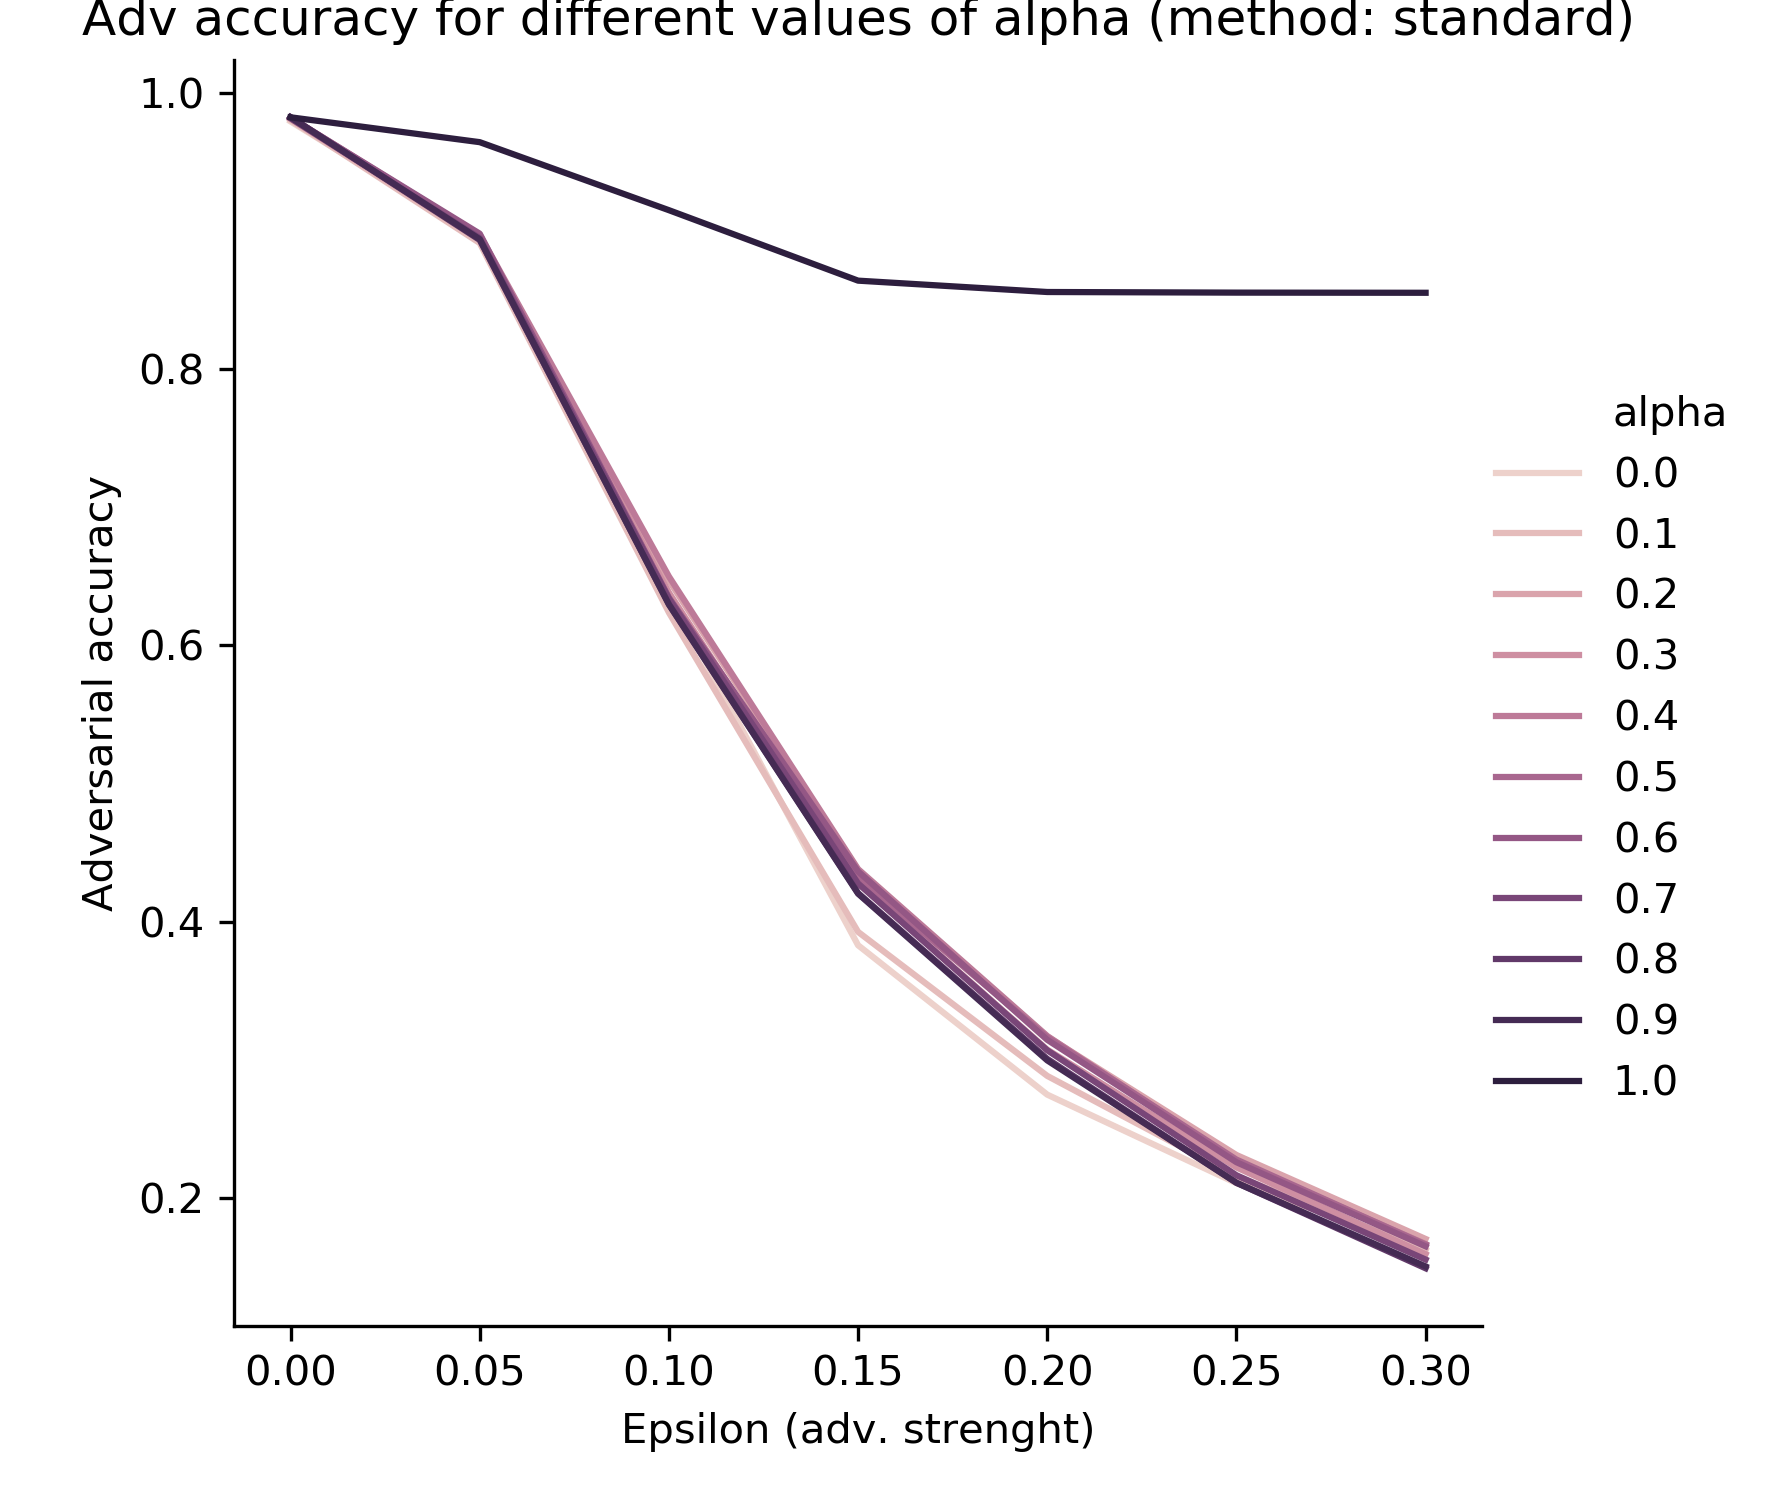
\includegraphics[scale=0.35]{adv_acc_std.png} }}%
    \quad
    \subfloat[BLS]{{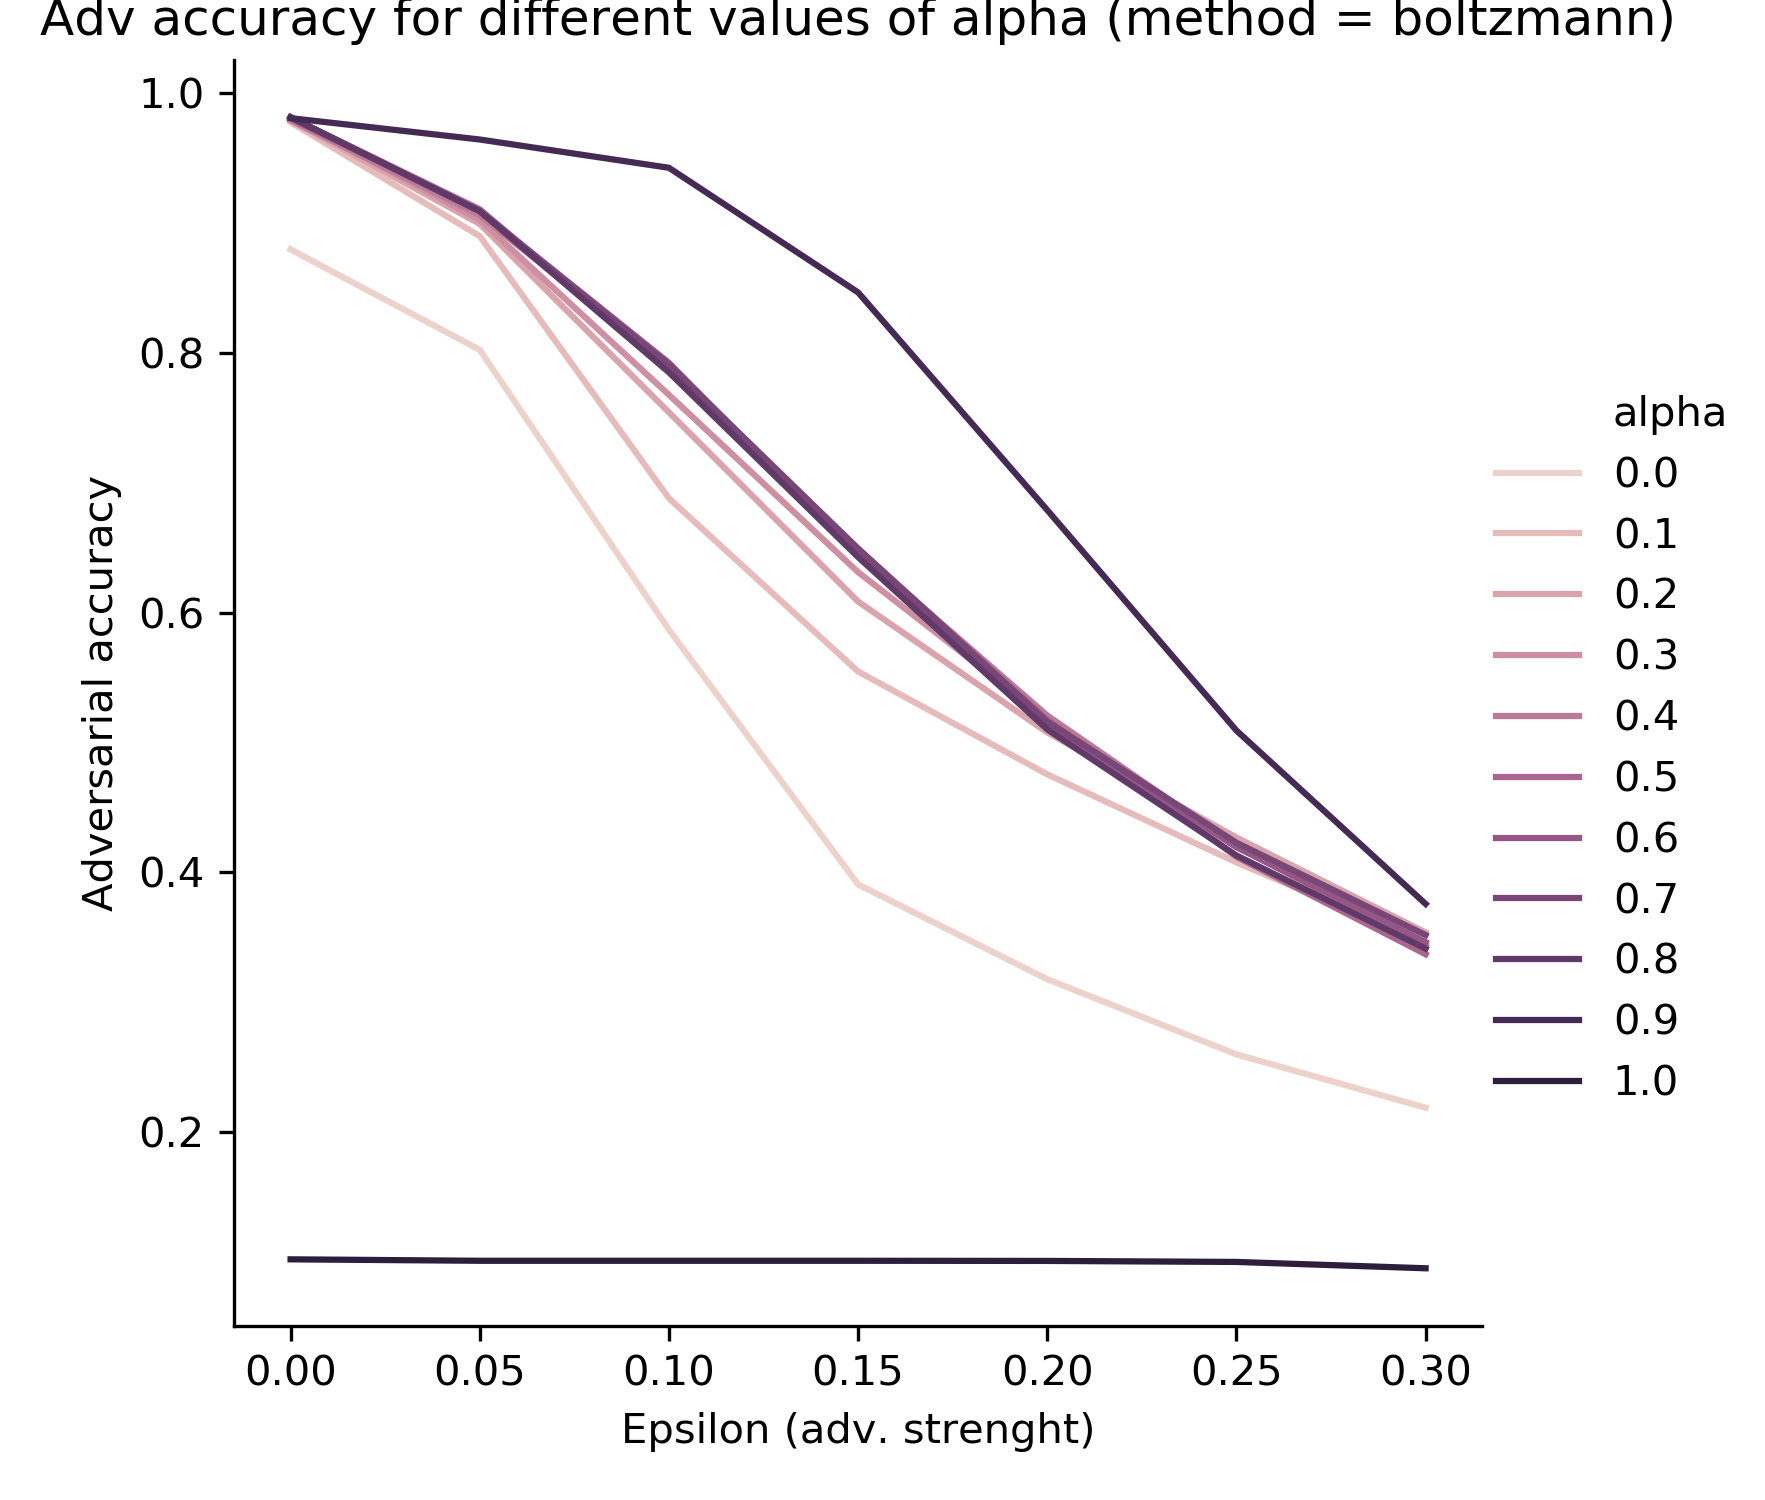
\includegraphics[scale=0.35]{adv_acc_boltzmann1.png} }}%
    \caption{Dataset: MNIST, attack method: FGSM. Adversarial accuracy using different label smoothing method.}%
    \label{fig:example}%
\end{figure}
\section{Conclusion}
...

\bibliographystyle{icml2017}
\bibliography{references}
\appendix
\section{Proofs}
\label{sec:proofs}
\begin{lemma}
Let  $\alpha \in [0, 1]$, $t \in [\![k]\!]$, and $g \in \mathbb R^k$. The
general solution of the problem
\begin{eqnarray}
  \underset{q \in \Delta_k,\, q^{(t)} \ge 1-\alpha}{\argmax}\; q^Tg
\end{eqnarray}
is $q^*=(1-\alpha) \delta_t + \alpha\bar{q}$, where $\bar{q}$ is any solution to
the problem with $\alpha=0$, namely $\bar{q} \in \argmax_{q \in \Delta_k}q^tg$
\label{thm:bumbednash}
\end{lemma}
\begin{proof}
Consider the invertible change of variable $x = h(\bar{x}):=\epsilon\delta_1 +
(1-\epsilon)\bar{x}$ which maps the simplex $\Delta_k$ unto itself, with inverse
$\bar{x} = h^{-1}(x)=(1-\epsilon)^{-1}(x-\epsilon\delta_1)$.

It follows, that
$$
\min_{x \in \Delta_k | x_1 \ge \epsilon}x^Tb=\min_{x \in \Delta_k |
  x-\alpha\delta_1 \ge
  0}x^Tb=\min_{(1-\epsilon)^{-1}(x-\epsilon\delta_1)}x^Tb=\min_{\bar{x} \in
  \Delta_k}(\epsilon\delta_1+(1-\epsilon)\bar{x})^Tb,
$$
which is attained by $\bar{x}^* \in \text{argmin}_{\bar{x} \in
  \Delta_k}\bar{x}^Tb=\text{ConvHull}(\text{argmin}_{j=1}^k b_j)$, yielding $
x^*=\epsilon\delta_1 + (1-\epsilon)\bar{x}^*$.
\end{proof}

\end{document}

